% Created 2016-12-29 Thu 18:28
\documentclass[11pt]{article}
\usepackage[utf8]{inputenc}
\usepackage[T1]{fontenc}
\usepackage{fixltx2e}
\usepackage{graphicx}
\usepackage{longtable}
\usepackage{float}
\usepackage{wrapfig}
\usepackage{rotating}
\usepackage[normalem]{ulem}
\usepackage{amsmath}
\usepackage{textcomp}
\usepackage{marvosym}
\usepackage{wasysym}
\usepackage{amssymb}
\usepackage{hyperref}
\tolerance=1000
\usepackage{minted}
\author{Gaurish}
\date{\today}
\title{r-Gather Programs}
\hypersetup{
  pdfkeywords={},
  pdfsubject={},
  pdfcreator={Emacs 24.5.1 (Org mode 8.2.10)}}
\begin{document}

\maketitle
\tableofcontents

\section{Introduction}
\label{sec-1}

The $r$-Gather problem was originally posed as a sub-problem in a \href{http://people.csail.mit.edu/karger/Papers/maybecast.pdf}{FOCS 2000} paper about constructing Steiner trees in 
the face of uncertainty. It was explored in detail by \href{http://static.googleusercontent.com/media/research.google.com/en//pubs/archive/41225.pdf}{Aggarwal et al. }who gave various hardness results and 
approximation algorithms in the setting of metric spaces. It is natural to study this problem and its variants 
in $\mathbb{R}^2$ by exploiting the extra structure available. 

In the main paper, we give approximation algorithms for the following problems:

\textbf{DYNAMIC $r$-GATHER:}      If the $(x,y)$ co-ordinates of the data-set are live and moving, how do we update 
$OPT$ efficiently? 

\textbf{DECENTRALIZED $r$-GATHER:} Say the data-set is spread among several data-banks. How do we compute $OPT$ 
with minimal co-ordination? 

\textbf{DECENTRALIZED DYNAMIC $r$-GATHER:}  What if the data is live, \uline{\emph{\textbf{and}}} the computation 
is required to be as decentralized as possible?  

The sections that follow give literate Python implementations of these algorithms \footnote{I'll be using the latest Anaconda installation of Python 2.7. Note that some older versions of Matplotlib give errors 
when trying to do the animation with generators as documented \href{https://github.com/matplotlib/matplotlib/pull/2634}{here}. However, the version of Matplotlib bundled up in Anaconda's latest Python 2.7+ environment does not have these problems} 

\section{About the Test Data}
\label{sec-2}
\href{./shenzhen_trajectory_data.png}{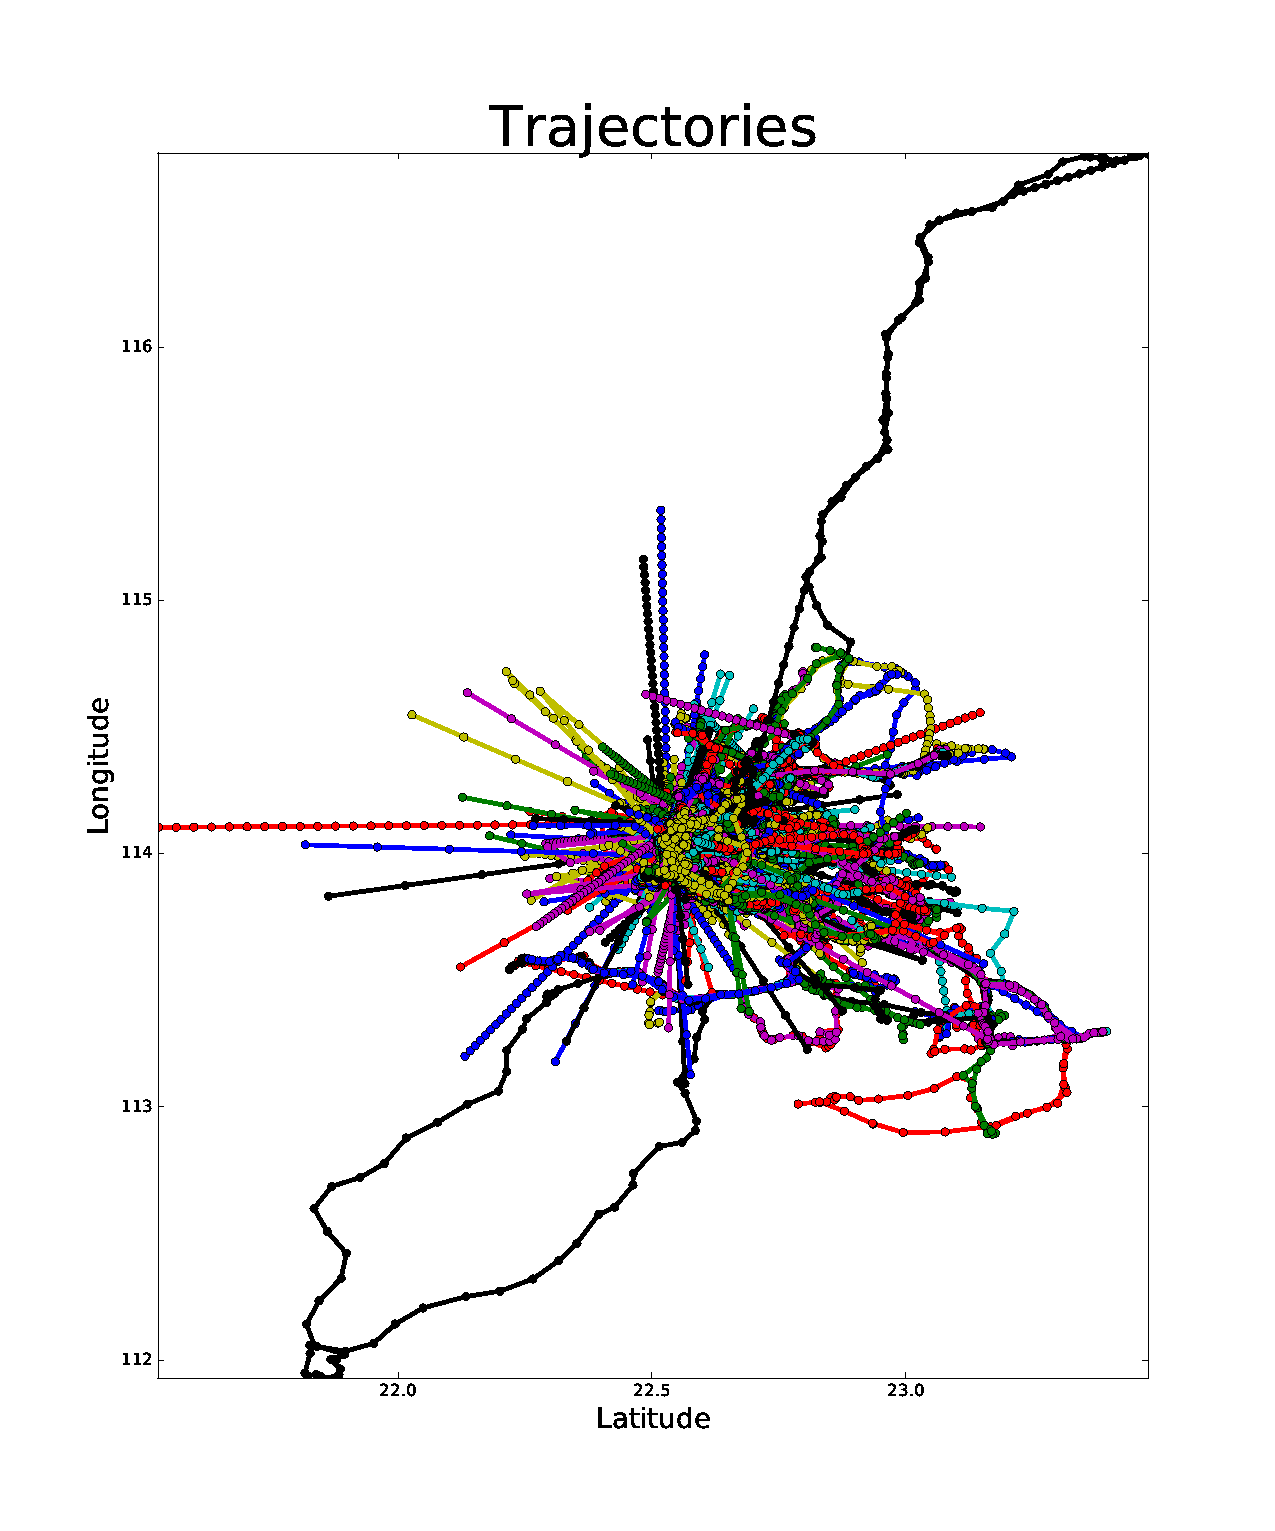
\includegraphics[width=.9\linewidth]{./InputOutput/shenzhen_trajectory_data.png}}
Figure 1 on the left depicts trajectories of 9386 cars, fitted with GPS sensors, driving 
around Shenzhen, China for a single day. \href{shenzen_normalized_data_animation_for_small_subset_of_cars.mp4}{Here} is a video of a small subset of them evolving in time.  

The GPS co-ordinates from the raw data set (consisting of latitude and longitude given in degrees) 
have been "normalized"; so we can assume the cars have been sampled in lock-step, every 5 minutes.

The goal of the $r$-Gather problem and its variants is -- broadly speaking -- to fuzz these trajectories for anonymity, 
yet still preserve enough structure to make useful inferences. 




\section{The Implementations}
\label{sec-3}
I will be implementing each of the five algorithms as classes in \textbf{\verb~rGather.py~}. These classes will behave as 
namespaces for different runs of the algorithms. \textbf{There will be no dependence between the classes}. That will 
allow us to unit-test them individually.  

Each class comes with its own  main.py   
file to customizing the needed logic. But the module file remains the same. I will not be documenting the 
logic of the \textbf{main.py} files in this literate document, for they are self-explanatory. 

The statistics of the clustering, on the other hand will be visualized by the \textbf{plotStatistics} method 
It will get its own axes artist object(s) on which to plot these statistics. 

I intend to use the classes as described below:

\begin{description}
\item[{\uline{Test the performance of various algorithms on a stored data-set}}] \begin{itemize}
\item Initialize \textbf{(but not necessarily start!)} one or more $r$-Gather routines with the input-data.
\item Every class has a method called \textbf{\verb~generateState({config})~} which runs the actual
algorithm on the provided input. The computed clusterings and statistics of the 
run are stored as member variables or maybe as a dictionary.
\item Each class also has one or more functions for visualizing the clusterings or 
run-time statistics so gathered.
\item The dynamic algorithms also come with one or more animation functions  
interacting with the \textbf{\verb~generateState()~} via the \textbf{\verb~yield~} statement and the 
\textbf{\verb~animation.FuncAnimation(..)~} HOF.
\item Every method itself will have routines local to its scope to help abstracting away its logic. 
Strive to make these local routines pure. Moreover, make all the needed module imports local.  
That will help us via property checkers or other unit-testing mechanisms.
\end{itemize}
\end{description}


\begin{description}
\item[{\uline{Stress test an algorithm adversarially via the little GUI}}] \begin{itemize}
\item The user enters the points by double-clicking on the canvas.

\item To set the $r$-parameter he will 
\begin{itemize}
\item Press \textbf{r} or \textbf{R} key
\item Then enter the decimal digits of this parameter.
\item After finishing, press enter, to execute the algorithm.
\end{itemize}

\item To clear the canvas and reset the algorithm class which is 
holding the state press \textbf{c} or \textbf{C} key.

\item Start inputting a new cloud of points to have a new run of the 
algorithm.
\end{itemize}
\end{description}

\rule{\linewidth}{0.5pt}

Finally, every run will need to record the statistics inside a YAML or an XML file. 
XML might be simpler if you will be using Beautiful soup. Besides the documents 
are far easier to view in the browser. YAML cannot be folded up unfortunately.
I will absolutely need the latter for viewing small-data-sets. 

There must be a function which produces this output! The following list should 
be produced for each point-cloud data-set. Note that the results from different 
clustering algorithms will be stored in the same file.   

\begin{description}
\item[{\uline{Static RGather}}] \begin{itemize}
\item Comment String. Allowed to be arbitrarily long.
\item The number of points
\item (x,y) coods of the points
\item List of clusterings computed different algorithms. 
$\forall$ clustering
\begin{itemize}
\item Algorithm Used
\item $r$ parameter
\item Number of clusters computed.
\item Now the actual clusters! 
$\forall$ clusters
\begin{itemize}
\item The number of points in the cluster
\item The diameter of the cluster
\item The actual points of the cluster.
\end{itemize}
\end{itemize}
\end{itemize}
\end{description}

We could stuff everything ever into one 
data-file but that would be too complicated! 




\subsection{The Main module file rGather.py}
\label{sec-3-1}

Here a bird's eye view of \textbf{rGather.py} after tangling.  

\begin{minted}[]{python}
#!/usr/bin/python
import matplotlib as mpl, numpy as np, scipy as sp, sys, math, colorsys 
from matplotlib import pyplot as plt, animation 
import networkx as nx, sklearn as sk
from abc import ABCMeta, abstractmethod
from haversine import haversine # https://pypi.python.org/pypi/haversine

<<ALGO_JIEMIN_DECENTRALIZED_STATIC>>

<<ALGO_AGGARWAL_STATIC>>
<<ALGO_AGGARWAL_STATIC_R2L2>> 

<<ALGO_JIEMIN_DYNAMIC>>

def getRandomColor():
    """ Ripped from http://goo.gl/SMlEaU"""

    golden_ratio_conjugate = 0.618033988749895

    h = np.random.rand() 
    h += golden_ratio_conjugate
    h %= 1.0
    return colorsys.hsv_to_rgb(h, 0.7, 0.9)
\end{minted}

\subsection{Decentralized Static $r$-Gather (4-Approx)}
\label{sec-3-2}


This algorithm is implemented as a class as described in the previous sections. Each instantiation 
is an "environment" in which the algorithm runs. To construct the class, we pass 
the cluster parameter $r$ and the co-ordinates of the point-cloud. Some of the class variables stores 
various statistics gathered while executing the algorithm on the given point cloud.

In the coming subsections, I'll describe each of the noweb references of the code-block below. 
These references are just the methods of this class grouped logically.  



\begin{minted}[]{python}
class AlgoJieminDecentralizedStatic:
    <<SETUP_AND_CLEANUP>>
    <<GENERATE_CLUSTERS>> 
    <<PLOT_CLUSTERS>>  
    <<PLOT_STATISTICS>>
\end{minted}

\subsubsection{Setup and Cleanup}
\label{sec-3-2-1}

This chunk is  self-explanatory. The constructor initializes state variables needed as input
along with data variables needed for a post-hoc analysis. These latter will be computed during the 
algorithm's run.  

Note that the final result of the clustering algorithm is stored in \textbf{self.computedClusterings},  
of type \textbf{\verb~[[Int]]~}, i.e. a list of list of indices. These indices correspond to the row-numbers 
of the \uline{input} numpy array \textbf{pointCloud}: each row in pointCloud corresponds to a point in $\mathbb{R}^2$. 

\begin{minted}[]{python}
def __init__(self, r, pointCloud):
  """  r          : Cluster parameter
       pointCloud : An n x 2 numpy array where n is the number 
                    of points in the cloud and each row contains 
                    the (x,y) coordinates of a point."""

  self.r                    = r     
  self.pointCloud           = pointCloud  
  self.computedClusterings  = []  
  self.algoName             = 'Decentralized Static r-Gather'



def clearAllStates(self):
  self.r                   = None
  self.pointCloud          = [] 
  self.computedClusterings = []


def clearComputedClusteringsAndR(self):
  self.r                   = None
  self.computedClusterings = []
\end{minted}

\subsubsection{Generate Clusters}
\label{sec-3-2-2}

The algorithm. Finally! Note that this method is NOT called by the constructor when initializing 
the class. This is by design to gain extra flexibility during experimental analyses. 


\begin{minted}[]{python}
def generateClusters(self, config={'mis_algorithm': 'networkx_random_choose_20_iter_best'}):
  """ config : Configuration parameters which might be needed 
               for the run. 
  Options recognized are (ALL LOWER-CASE)
  1. mis_algorithm:
       A. 'networkx_random_choose_20_iter_best', default 
       B. 'riksuggestion'
  """


  import itertools
  import numpy as np
  import pprint as pp
  import copy
  <<FIND_NEAREST_NEIGHBOURS>>
  <<FIND_MAXIMAL_INDEPENDENT_SET_NEIGHBOURHOODS>>
  <<EXTRACT_UNIQUE_ELMENTS_FROM_LIST>>
  <<DISTANCE_FUNCTION>>


  NrDistances, Nr = findNearestNeighbours( self.pointCloud, 
                                           self.r )
  S               = findMaximalIndependentOfNeighbourhoods( Nr.tolist( ), 
                                                            config[ 'mis_algorithm' ] )

  indicesOfPointsCoveredByS = set(list(itertools.chain.from_iterable(S)))
  indicesOfPointsMissedByS  = set(range(len(self.pointCloud))).difference(indicesOfPointsCoveredByS)

  assert(indicesOfPointsCoveredByS.union(indicesOfPointsMissedByS ) == set(range(len(self.pointCloud))) )

  # For each point missed by S, find which elements of its r-neighbourhood lies inside a member of S. 
  pNrS = {} # A dictionary which maintains this information.  
  for index in indicesOfPointsMissedByS:

     pNrS[index] = [] 

     #Coordinates of the point whose index is 'index'
     ptIndex     = np.array( self.pointCloud[index] )

     neighborIndices = Nr[index][1:] 

     for nbIndex in neighborIndices:
       for s in S:
         if nbIndex in s:

           ptnbIndex = np.array(self.pointCloud[nbIndex])

           dist = np.linalg.norm( ptIndex - ptnbIndex  ) # Euclidean distance between the points
           pNrS[index].append(  (s, dist)    )
           break # since members of S are disjoint there is no reason to continue to iterate over members of S to check containment of nbindex
                 # Move onto the next member of neighbourIndices. 

  # print "\nNr   = "     , Nr
  # print "\nS    = "     , S
  # print "\npointsMissed", indicesOfPointsMissedByS
  # print "\npNrS = "     ; pp.pprint(pNrS, width=20 )


  # Now for each point select the member of S that is closest using this dictionary. 
  # Edit this dictionary in place, by keeping only the closest neighbourhood. 
  pNrS_trimmed = {}
  for (key, value) in pNrS.iteritems():
      distmin = float("inf") # Positive infinity

      for (s, dist) in value:
        if dist<distmin:
            smin    = s
            distmin = dist


      #pNrS_trimmed[key] = (smin,distmin) # For debugging purposes. 
      pNrS_trimmed[key] = smin

  #print "\npNrS_trimmed = "; pp.pprint(pNrS_trimmed, width=1) 



  # With pNrS_trimmed we obtain the final clustering. Yay!
  # by "inverting" this key-value mapping
  augmentedSets = [s for s in S if s not in pNrS_trimmed.values()] # The sets just included are not augmented at all. 

  pNrS_codomain = extractUniqueElementsFromList(pNrS_trimmed.values())

  for s in pNrS_codomain:
    smodified = copy.copy(s) # This copying step is SUPER-CRUCIAL!!! if you just use =, you will just be binding object pointed to by s to smod. Modifying smod, will then modify s, which will trip up your future iterations! I initially implemented it like this and got tripped up 
    for key, value in pNrS_trimmed.iteritems():
      if s == value:
        smodified.append(key) # augmentation step

    augmentedSets.append(smodified)


  self.computedClusterings = augmentedSets

  #print "\nself.computedClusterings = "; pp.pprint(self.computedClusterings,width=1)
  print   "Numpoints = "                   , len( self.pointCloud )       ,  \
          " r = "                          , self.r                       ,  \
          " Number of Clusters Computed = ", len( self.computedClusterings ), \
          " Algorithm used: "              , self.algoName
  sys.stdout.flush()
\end{minted}



The noweb references above are helper functions which I'll describe next. 

\textbf{\uline{FIND NEAREST NEIGHBOURS}}

Given a point-cloud, the following function computes the $k$-nearest neighbours of each 
point and their corresponding distances as required by \textbf{generateClusters}. 


 \textbf{\uline{WARNING!}} The neighbour list as computed here consist of the 0th, 1st, 2nd, \ldots{}., 
(k-1)th nearest neighbours. The 0th neighbour is a hack, which allows us to identify 
the point about whose neighbour list we are talking about. 

\begin{minted}[]{python}
def findNearestNeighbours(pointCloud, k):
  """  pointCloud : 2-d numpy array. Each row is a point
       k          : The length of the neighbour list to compute. 
  """
  from sklearn.neighbors import NearestNeighbors
  import sklearn
  import numpy as np
  import sys



  X    = np.array(pointCloud)
  nbrs = NearestNeighbors(n_neighbors=k, algorithm='ball_tree').fit( X )
  distances, indices = nbrs.kneighbors(X)

  return distances, indices
\end{minted}

The output variable is a list of neighbour-lists reported by sklearn: $N[i]$ denotes the \textbf{index-list} of the 
$k$-nearest neighbours of point $i$. The indices are specified in increasing order of distance of the corresponding 
points from point i. 

$NDistances[i]$ is the corresponding list of distances of the $k$-nearest neighbours of point $i$. 

In particular, $N[i][j]$ and $NDistances[i][j]$ \uline{\textbf{respectively}} denote the index of \uline{and} distance between the $j$ th nearest 
neighbour of $i$. 


\uline{\textbf{FINDING A MAXIMAL INDEPENDENT SET OF NEIGHBOURHOODS}}


Given a collection of point-sets in the plane, we can use networkX to extract a large maximally independent -- wrt intersection--
subcollection. 

For that, I construct a graph where 
\begin{enumerate}
\item Each point-set corresponds to a vertex in the graph and vice-versa
\item There exists an edge between two vertices in the graph if and only if, 
the corresponding point-sets have a non-empty intersection.
\end{enumerate}

\begin{minted}[]{python}
def findMaximalIndependentOfNeighbourhoods(  nbds , mis_algorithm  ):
  import networkx as nx
  G = nx.Graph()
  G.add_nodes_from(range(len(nbds)))

  # If two neighbourhoods intersect, draw 
  # a corresponding edge in the graph. 
  for i in range(len(nbds)):
    for j in range(i+1,len(nbds)):
      intersection_of_nbds_ij = [  val  for val in nbds[i] if val in nbds[j]    ] 
      if len(intersection_of_nbds_ij) >= 1:
        G.add_edge(i,j)

  # Having constructed the neighbourhood, we proceed to find a good MIS
  # The quality of the solution is affected by the size of the MIS
  # The larger the maximal independent set, the better it is
  if mis_algorithm == 'networkx_random_choose_20_iter_best': 
    candidateSindices = [ nx.maximal_independent_set(G) for i in range(20)  ]

    #for candidate in candidateSindices: # for debugging
    #  print candidate

    sIndices = [] # Start value for finding the maximum
    for candidate in candidateSindices: # Pick the largest independent set over 10 iterations
      if len(candidate) > len(sIndices): # Yay! Found a larger independent set!
        print "Larger set!"
        sIndices = candidate


  elif mis_algorithm == 'riksuggestion':

    # Give cluster centers a special attribute marking it as a center. 
    distanceFromRthNearestNeighbourDict = {}

    for nbd, i in zip( nbds, range( len(nbds) )): # Note that each neighbourhood's 0th element is the center, and that the nbd indices are sorted by distance from this zeroth element. So -1 makes sense
        nbdCenterCoords                      = self.pointCloud[ nbd[0] ] 
        nbdFarthestNeighbourCoords           = self.pointCloud[ nbd[-1] ]
        distanceFromRthNearestNeighbourDict[i] = np.linalg.norm( [ nbdCenterCoords[0] - nbdFarthestNeighbourCoords[0] ,
                                                                   nbdCenterCoords[1] - nbdFarthestNeighbourCoords[1] ]  )# Abstract this away with the distance function later. 

    nx.set_node_attributes( G, 'distanceFromRthNearestNeighbour', distanceFromRthNearestNeighbourDict )

    import collections
    # Generate the order to remove the vertices
    orderOfVerticesToDelete = collections.deque(sorted(  range(len(nbds)) , key = lambda x: G.node[x][ 'distanceFromRthNearestNeighbour' ]    ))

    #print orderOfVerticesToDelete
    #for i in orderOfVerticesToDelete:
    #  print G.node[i]['distanceFromRthNearestNeighbour']
    sIndices = [ ]


    for i in orderOfVerticesToDelete:

      try:
         node = orderOfVerticesToDelete[i]

         nlist = G.neighbors( node )

         for n in nlist:
           try:
             G.remove_edge( node, n ) # Remove all edges emanating
           except nx.NetworkXError:
             continue

         G.remove_node( node ) # Remove the node itself


         for n in nlist:
           try:
             G.remove_node( n ) # Remove all the neighbours.
           except nx.NetworkXError:
             continue

         sIndices.append( node ) 

      except nx.NetworkXError:
          continue


    # while( len( orderOfVerticesToDelete ) >= 1 ): # This list changes during the iteration. 

    #     try:
    #       node  = orderOfVerticesToDelete[0]

    #     except nx.NetworkXError:
    #         print "Removing carcass"
    #         orderOfVerticesToDelete.popleft()

    #     else:
    #       sIndices.append( node ) # The very fact no exception was thrown means that you can freely add it to the independent set
    #       nlist = G.neighbors( node )

    #       # Delete all the edges emanating from  elements of nlist. 
    #       # The fact that this did not throw an exception means 'node' still exists in the graph G
    #       for n in nlist:
    #          G.remove_edge( node, n ) # Remove all edges emanating

    #       G.remove_node( node ) # Remove the node itself

    #       for n in nlist:
    #         G.remove_node( n ) # Remove all the neighbours.

    #       orderOfVerticesToDelete.popleft()

  else:
    import sys
    print "Maximum independent Set Algorithm option not recognized!"
    sys.exit()


  # If two neighbourhoods intersect, draw 
  # a corresponding edge in the graph. 
  # print sIndices
  for i in sIndices:
     for j in sIndices:
       if j > i:
         intersection_of_nbds_ij = [val for val in nbds[i] if val in nbds[j] ]
         if len(intersection_of_nbds_ij) >= 1:
               print "Neighbourhoods intersect!"
               sys.exit()

  # print "Exiting!"
  # import sys
  # sys.exit()

  return [ nbds[s] for s in sIndices ]
\end{minted}


\begin{minted}[]{python}
def extractUniqueElementsFromList( L ):

    uniqueElements = []
    for elt in L:
        if elt not in uniqueElements: # Just discovered a brand new element!!
            uniqueElements.append(elt)

    return uniqueElements
\end{minted}



\subsubsection{Plot Clusters}
\label{sec-3-2-3}

Once the clustering has been constructed we can now visualize it.This function in particular will continue to be in flux: 
so I'll let the code do the talking here. Just note that the algorithm object does not store a reference to the axes object 
on which the clusterings will be plotted. Hence we have to explicitly pass the axes object when calling this method. 
.   This is a conscious design goal!  'Twill help us in visually comparing the 
cluters outputted by the different approximation algorithms for the same problem. Depending on the algorithms to be compared 
construct a fig object with multiple axes objects. Then each visualization routine of an algorithm gets an axes-object 
reference from this figure. 


\begin{minted}[]{python}
def plotClusters(self,  ax    , 
               pointSize=200, 
               marker='o'   , 
               pointCloudInfo='',
               annotatePoints=True):


      from scipy import spatial
      import numpy as np, matplotlib as mpl
      import matplotlib.pyplot as plt

      # Plot point-cloud 
      xs = [x for (x,y) in self.pointCloud]
      ys = [y for (x,y) in self.pointCloud]
      ax.plot(xs,ys,'bo', markersize=3) 
      ax.set_aspect(1.0)    

      if annotatePoints==True:
            # Annotate each point with a corresponding number. 
            numPoints = len(xs)
            labels = ['{0}'.format(i) for i in range(numPoints)]

            for label, x, y in zip(labels, xs, ys):
                  ax.annotate(  label                       , 
                                xy         = (x, y)         , 
                                xytext     = (-3, 0)      ,
                                textcoords = 'offset points', 
                                ha         = 'right'        , 
                                va         = 'bottom')


      # Overlay with cluster-groups.
      for s in self.computedClusterings:

        clusterColor = getRandomColor()
        xc = [ xs[i]  for i in s   ]
        yc = [ ys[i]  for i in s   ]

        # Mark all members of a cluster with a nice fat dot around it. 
        #ax.scatter(xc, yc, c=clusterColor, 
        #           marker=marker, 
        #           s=pointSize) 

        #ax.plot(xc,yc, alpha=0.5, markersize=1 , markerfacecolor=clusterColor , linewidth=0)
        #ax.set_aspect(1.0)

        # For some stupid reason sp.spatial.ConvexHull requires at least three points for computing the convex hull. 

        if len(xc) >= 3 : 
              hull = spatial.ConvexHull(  np.array(zip(xc,yc)) , qhull_options="QJn" ) # Last option because of this http://stackoverflow.com/q/30132124/505306
              hullPoints = np.array( zip( [ xc[i] for i in hull.vertices ],  
                                          [ yc[i] for i in hull.vertices ] ) )
              ax.add_patch( mpl.patches.Polygon(hullPoints, alpha=0.5, 
                                                facecolor=clusterColor) )


        elif len(xc) == 2:
               ax.plot( xc,yc, color=clusterColor )


        ax.set_aspect(1.0)
        ax.set_title( self.algoName + '\n r=' + str(self.r), fontdict={'fontsize':5})
        ax.set_xlabel('Latitude', fontdict={'fontsize':5})
        ax.set_ylabel('Longitude',fontdict={'fontsize':5})

        #ax.get_xaxis().set_ticks( [] ,  fontdict={'fontsize':10})
        #ax.get_yaxis().set_ticks( [],  fontdict={'fontsize':10} ) 

        ax.grid(b=True)
\end{minted}





\subsubsection{Plot Statistics}
\label{sec-3-2-4}

Axes artist objects are Hashable! We use this to get a lot of flexibility 
during plotting! I verified this using this answer \url{http://stackoverflow.com/a/3460747/505306} 

The nice thing about these statistics, are that they along with cluster sizes, can be rendered 
online as we keep filling in more and more points by appropriate bindings to button press events. 

\begin{minted}[]{python}
def plotStatistics(self, axStatsDict ):
   """ axStatsDict, specifies the mapping of axes objects to the statistic
       being plotted.""" 

   def plotConvexHullDiameters(ax):
      pass

   def plotMinBoundingCircleDiameters(ax):
      pass

   def plotClusterPopulationSizes(ax):
      barHeights = map(len, self.computedClusterings )
      numBars    = len(barHeights)

      ax.bar( range(numBars) ,barHeights, width=1.0, align='center')
      ax.set_title('Number of points per Cluster', fontdict={'fontsize':30})

      ax.set_aspect(1.0)
      ax.grid(b=True)

   for ax, statistic in axStatsDict.iteritems():

        if statistic == 'convexHullDiameters': 
           plotConvexHullDiameters(ax) 

        elif statistic == 'minBoundingCircleDiameters':
           plotMinBoundingCircleDiameters(ax)

        elif statistic == 'clusterPopulationSizes':
           plotClusterPopulationSizes(ax)

        else:
           pass
\end{minted}





\subsection{Aggarwal's Static $r$-Gather (2-Approx)}
\label{sec-3-3}
Since the algorithm can work for any metric space, I'll implement it as an abstract 
base class called \textbf{\verb~AlgoAggarwalStatic~}. For a specific metric-space, it will run as a 
method in a subclass of this ABC. This sub-class will implement the distance 
function and other visualization routines and possibly faster neighbour search routines
than the default one provided in the base class viz. that of the brute force quadratic
search. You might even want to consider making this neighbour search an abstract method 
when dealing with trajectory data. 

The following code block are birds-eye views of \textbf{\verb~AlgoAggarwalStatic~} and \textbf{\verb~AlgoAggarwalR2L2~}. 
\begin{minted}[]{python}
class AlgoAggarwalStatic:
  __metaclass__ = ABCMeta

  def __init__(self,r,pointCloud):
    """ Even though this is an abstract class, a subclass is 
        allowed to call the constructor via super. 
        However, a user cannot instantiate a class with this 
        method from his code."""
    pass 


  @abstractmethod
  def dist(p,q):
    """ A distance function of a metric space.
        distance between points p and q. Implemented 
        by the subclass. """
    pass

  @abstractmethod
  def rangeSearch( pointCloud, radius):
    """ Given a set of points in the metric space, and a radius value
        find all the neighbours for a point in 'pointCloud' in a ball of radius, 
        'radius', for all points in 'points'. Depending on the metric space 
        an efficient neighbour search routine will use different tricks """ 
    pass 

  <<GENERATE_CLUSTERS_AGGARWAL>>
\end{minted}


The following concrete class inheriting from \textbf{\verb~AlgoAggarwalStatic~} is implemented for the trajectory case
\begin{minted}[]{python}
class AlgoJieminDynamic( AlgoAggarwalStatic ):

    def __init__(self, r,  pointCloud):
       # len(trajectories) = number of cars
       # len(trajectories[i]) = number of GPS samples taken for the ith car. For shenzhen data set this is
       # constant for all cars.

       self.r                    = r     
       self.pointCloud           = pointCloud # Should be of type  [ [(Double,Double)] ] 
       self.computedClusterings  = []  
       self.algoName             = 'r-Gather for trajectory clustering'


    def clearAllStates(self):
          self.r                   = None
          self.pointCloud          = [] 
          self.computedClusterings = []

    def clearComputedClusteringsAndR(self):
             self.r                   = None
             self.computedClusterings = []

    def dist(self, p,q):
       """ distance between two trajectories p and q. The trajectories form a metric space under this distance 
       If you visualize the given table as a microsoft excel sheet, where each column represents the trajectory 
       of a car, then the distance between two trajectories is the max of L infinity norm of the difference of two 
       columns. 

       p,q :: [(Double,Double)]. The length of p or q, indicates the number of GPS samples taken

       """
       dpq = 0
       for t in range(len(p)):

            # M is the euclidean distance between two points at time t.  
            M = np.sqrt( abs( (p[t][0]-q[t][0])**2 + (p[t][1]-q[t][1])**2 ) ) 
            if M > dpq:
                dpq = M

       return dpq


    def findNearestNeighbours(self, pointCloud, k):
       """Dumb brute force nearest neighbours"""
       import numpy as np
       import sys
       # return distances, indices

       distances = []
       indices   = []
       for traj_i, i in pointCloud, range(len(pointCloud)):
              distances_and_indices = []
              for traj_j, j in pointCloud, range(len(pointCloud)):
                    dij = self.dist( traj_i, traj_j)
                    distances_and_indices.append[(dij,j)]

              # Now sort the distances of all points from point i. 
              distances_and_indices.sort(key=lambda tup: tup[0]) # http://tinyurl.com/mf8yz5b
              distances.append( [ d for (d,i) in distances_and_indices[0:k] ]  )
              indices.append  ( [ i for (d,i) in distances_and_indices[0:k] ]  )

       print "Fuck you!"
       return distances, indices


    def rangeSearch(self, pointCloud, radius):
        print "Warning! Rangesearch used for trajectories"
        pass


    <<PLOT_CLUSTERS>>
    <<PLOT_STATISTICS>>
\end{minted}







The following concrete class inheriting from \textbf{\verb~AlgoAggarwalStatic~} is implemented for the $L^2$ metric
in $\mathbb{R}^2$

\begin{minted}[]{python}
class AlgoAggarwalStaticR2L2( AlgoAggarwalStatic ):

   def __init__(self, r, pointCloud):

      self.r                    = r     
      self.pointCloud           = pointCloud 
      self.computedClusterings  = []  
      self.algoName             = 'Metric Space Static r-Gather applied to R2L2'

      #super(  AlgoAggarwalStaticR2L2, self ).__init__( self.r, self.pointCloud  )

   def clearAllStates(self):
         self.r                   = None
         self.pointCloud          = [] 
         self.computedClusterings = []

   def clearComputedClusteringsAndR(self):
            self.r                   = None
            self.computedClusterings = []

   def dist(self, p,q):
      """ Euclidean distance between points p and q in R^2 """
      return np.linalg.norm( [ p[0]-q[0] , 
                               p[1]-q[1] ]  )


   def findNearestNeighbours(self,pointCloud, k):
      """  pointCloud : 2-d numpy array. Each row is a point
      k          : The length of the neighbour list to compute. 
      """
      from sklearn.neighbors import NearestNeighbors
      import numpy as np
      import sys

      X    = np.array(pointCloud)
      nbrs = NearestNeighbors(n_neighbors=k, algorithm='ball_tree').fit(X)
      distances, indices = nbrs.kneighbors(X)

      return distances, indices


   def rangeSearch(self, pointCloud, radius):
      """ A wrapper for a good neighbour search routine provided by Scipy.
          Given a point-cloud, return the neighbours within a distance of 'radius'
          for every element of the pointcloud. return the neighbour indices , sorted 
          according to distance. """
      import numpy as np
      import sys
      from scipy import spatial

      X        = np.array( pointCloud )
      mykdtree = spatial.KDTree( X )
      nbrlists = list( mykdtree.query_ball_point( X, radius) )


      distances = []
      for index  in  range(len(nbrlists)):

         def fn_index( i ): # Distance function local to this iteration of the loop
            return np.linalg.norm(  [  X[i][0] - X[index][0]   , 
                                       X[i][1] - X[index][1]    ]    )

         # Replace the unsorted array with the sorted one. 
         nbrlists[index]  = sorted( nbrlists[index], key = fn_index  ) 

         # Get corresponding distances, which will now naturally be in sorted order. 
         distances.append( map( fn_index, nbrlists[ index ] ) ) 


      indices = nbrlists # Just a hack, too lazy to change nbrlists to the name indices above. 

      return distances, indices 


   <<PLOT_CLUSTERS>>
   <<PLOT_STATISTICS>>
\end{minted}

\textbf{IMPORTANT NOTE!}
The same exact methods for plotting the clusters and various other statistics from AlgoJieminDecentralizedDynamic
will apply here, so I'll just use a noweb-ref to insert them verbatim. In fact, they SHOULD be exactly the same 
for comparing AlgoJiemin and AlgoAggarwal. The noweb-references ensure we don't need to manually make the 
same changes in both classes. 


\subsubsection{Generate Clusters}
\label{sec-3-3-1}
\verb~<<GENERATE_CLUSTERS_AGGARWAL>>~ expands to the \textbf{\verb~generateClusters~} method which implements the actual algorithm.  

\begin{minted}[]{python}
def generateClusters(self):
  from   colorama import Fore, Style 
  import pprint as pp 
  import networkx as nx, numpy as np, random, time 
  import scipy as sp
  import matplotlib.pyplot as plt
  import sys
  points    = self.pointCloud # a conveninent alias 
  numPoints = len( self.pointCloud )

  <<FIRST_CONDITION_PREDICATE>>
  <<MAKE_CLUSTER_CENTERS>> # There are two such assumptions. 
  <<MAKE_FLOW_NETWORK>>
  <<MAKE_AGGARWAL_CLUSTERS>>

  print "Started filtering!"

  dijHalfs = [0.5 * self.dist( points[ i ], points[ j ] ) 
                    for i in range( numPoints ) 
                    for j in range( i+1, numPoints ) ]
  # Find all dijs satisfying condition 1 on page 4

  print "dijhalfs computed", len(dijHalfs)
  dijHalfsFiltered =  filter( firstConditionPredicate, dijHalfs )  #smallest to highest
  print "dijHalfsFiltered done!"

  # 'FOR' Loop to find the minimum 'R' from these filtered dijs satisfying 
  #  condition 2 on page 4 of the paper. 
  bestR, bestRflowNetwork, bestRflowDict = float( 'inf' ), nx.DiGraph(), {} 
  bestRCenters = []

  for R in dijHalfsFiltered : # The first R that goes through the else block is the required R

    clusterCenters = makeClusterCenters( R )
    flowNetwork    = makeFlowNetwork( R, clusterCenters )

    try: # Check if a feasible flow exists in the constructed network.  
          flowDict = nx.min_cost_flow( flowNetwork )

    except nx.NetworkXUnfeasible:# If not, try the next R
          print Fore.RED, "Unfeasible R detected: R= ", R, Style.RESET_ALL
          continue 
    else: # Found a feasible R.  
        print "Found a feasible R! R= ", R
        if R < bestR: # Yippee a smaller and feasible R! Update bestR. 
            print Fore.RED, " In fact, it is the best thus far ", Style.RESET_ALL 
            bestR            = R
            bestRflowNetwork = flowNetwork
            bestRflowDict    = flowDict
            bestRCenters     = clusterCenters


  #Use the best network to construct the needed clusters. 
  self.computedClusterings = makeClusters( bestRflowDict, bestRCenters, bestRflowNetwork, R)

  # Sanity check on the computed clusters. They should all be of size r and should cover the full point set
  assert( all( [ len(cluster) >= self.r for cluster in self.computedClusterings ] ) )
  assert( len( { i for cluster in self.computedClusterings for i in cluster } ) == numPoints   )
  print Fore.YELLOW, "Yay All points Covered!!", Style.RESET_ALL

  print "BestRCenters are ", bestRCenters 
  return  bestRCenters
\end{minted}



The noweb-reference makeClusterCenters expands to the function definition given below. Neighbours of a point within
the distance $2R$ are chosen naively simply by iterating over the point cloud. I don't know how to do subquadratic 
time neighbour searches in general metric spaces. 

\emph{\textbf{NOTE} :: It is not immediately clear why the \verb~while~ loop below \textbf{must} terminate. Aggarwal et al.  do not prove this statement.  Possible 
 issue to be raised with Prof. Gao and Rik? But I suppose it might work for low values\ldots{}.$r = 2,3$\ldots{}Not sure.Will need to check this out properly.}
\emph{Possible hacks: if the loop looks like it is infinite, terminate it, and figure out how to treat these points.}


\section{Scrap notes}
\label{sec-4}
\begin{itemize}
\item Selecting an arbitrary submatrix of numpy.
\end{itemize}

\subsection{Animation in Python}
\label{sec-4-1}
For pulleys I did not use the animation module. Here we do since we need to understand the decision the algorithm
makes as the cars move along the trajectories.m 


\subsubsection{animation.FuncAnimation (\ldots{})}
\label{sec-4-1-1}
Generate the ith frame of an animation sequence. Thus you could say, its signature is \verb~Int -> IO Frame~ where 
Frame is the final picture returned.  

MAtplotlib can save video as an html5 video!! Basically all you need to do is provide an .mp4 or .ogg video
in the h264 encoding HTML5 format. It spits out a long hexadecimal like string.  
Then every browser (major ones atleast) will be able to play that video 
with their own media player which comes inbult. This means you don't need to distribute copies of vlc to other
people, neither upload that video to youtube and then emebed it. Yay!! 
See this video to customize the embedding: \url{https://www.youtube.com/watch?v=9pN7UT5S64I}


Essentially you surround the video link in the video tag, with some extra attributes. See here for a classic example! 
See the browser support table in the middle of this page: \url{http://www.w3schools.com/html/html5_video.asp} 
Plays on iPhone/iPad devices too!

See this for more on MATPLOTLIB html5 embedding: \url{http://yt-project.org/doc/cookbook/embedded_webm_animation.html}

\subsubsection{Data structures}
\label{sec-4-1-2}
Each trajectory shuld be a class. 
There should a distance function between two trajectories accepting them

\section{Types and Typeclasses}
\label{sec-5}


\section{Scrap}
\label{sec-6}

\section{Things to do for the dynamic rGather program}
\label{sec-7}
\begin{itemize}
\item $\boxtimes$ Make a main file from the animation file
\item $\boxtimes$ Go through the visualization routine. Adapt it to the visualization 
for this case.
\item $\boxtimes$ Add another class which derives from the metric space class
\item $\square$ Implement the 0 regroupings allowed. k passed as a parameter.
\item $\square$ Visualize the trajectories statically. Trajectories in a cluster are colored with the same color.
\item $\square$ Use the Delaunay triangulation heuristic for the r=3 case
\begin{itemize}
\item $\square$ Learn how to use delauny triangulation. Scipy has a routine
\item $\square$ I know how to use Linear Programming already. Just replace it with 
a linear program. USeful to understand the LP relaxation of it though. 
But if needed you can directly use your LP setcover heuristic that 
you implemented in here.
\end{itemize}
\item $\square$ Implement the epsilon kernel routine. 
\begin{itemize}
\item $\square$ It would be extremely useful to make a gridding function. 
You had implemented a similar one, in C++ some time back. 
Basically I think you would perform bucketing. \textbf{Add this to pointLib.py}
the library you wrote which handles interactive stuff, and can be appended 
to algorithms.
\item $\square$ This is a very simple algorithm. The only complex 
part is setting the parmaters
\item $\square$ The epsilon kernel routine is implemented as part of 
a new aproximate rGather algorithm with the same 
structure as wht you did before. The only twist, 
would be that you generate the clusters, by passing an 
additional parameter, which is the approximation parameter 
called epsilon.
\item $\square$ Have statistics to record the statistics of the sizes of the 
coresets, and other such trivia.
\end{itemize}
\item $\square$ Get properties of the proposed rGather coreset algorithm 
which uses onion layers.
\item $\square$ This can be easily implemented in an interactive frame 
by adapting the routine AlgoJieminDecentralizedStatic.
\item $\square$ The recursive improvement step, I think will be crucial to 
get improved results. Don't neglect the importance of this step.
\end{itemize}
% Emacs 24.5.1 (Org mode 8.2.10)
\end{document}
